\section{Early Results}

pytokio provides connectors for the following tools either available as community-supported open-source tools or pre-installed on Cray systems:

\begin{itemize}
\item \textbf{Cray SDB} for node topology
\item \textbf{Slurm} for job ID and node list mappings
\item \textbf{Darshan} for application-level I/O profiling
\item \textbf{Lustre} \texttt{lfs} and \texttt{lctl} for file system health
\item \textbf{LMT} for server-side Lustre loads via the ClusterStor Lustre monitoring tool~\cite{Keopp2014}
\end{itemize}

An example of a TOKIO analysis application is pytokio's Unified Monitoring and Metrics Interface (UMAMI)~\cite{Lockwood2017} application, which connects the aforementioned tools to visualize I/O performance alongside other dimensions of system health and contention.  Figure \ref{fig:umami} demonstrates the output of UMAMI in a case where poor performance on November 14 coincided with significant server-side bandwidth contention, OSS CPU load, and metadata contention.  As will be detailed further, aligning performance data from Darshan with Lustre server-side data from LMT allows users to see how each I/O subsystem component affects performance for their jobs.
% * <pcarns@gmail.com> 2018-01-19T16:21:36.773Z:
% 
% It seems like there should be some lead in text before the "Using these connectors" sentence to tie this text back to the four logical layers described earlier.  UMAMI and the heatmap thing are examples of "analysis applications" in that taxonomy, right?
% 
% ^.

\begin{figure}[t]
    \centering
    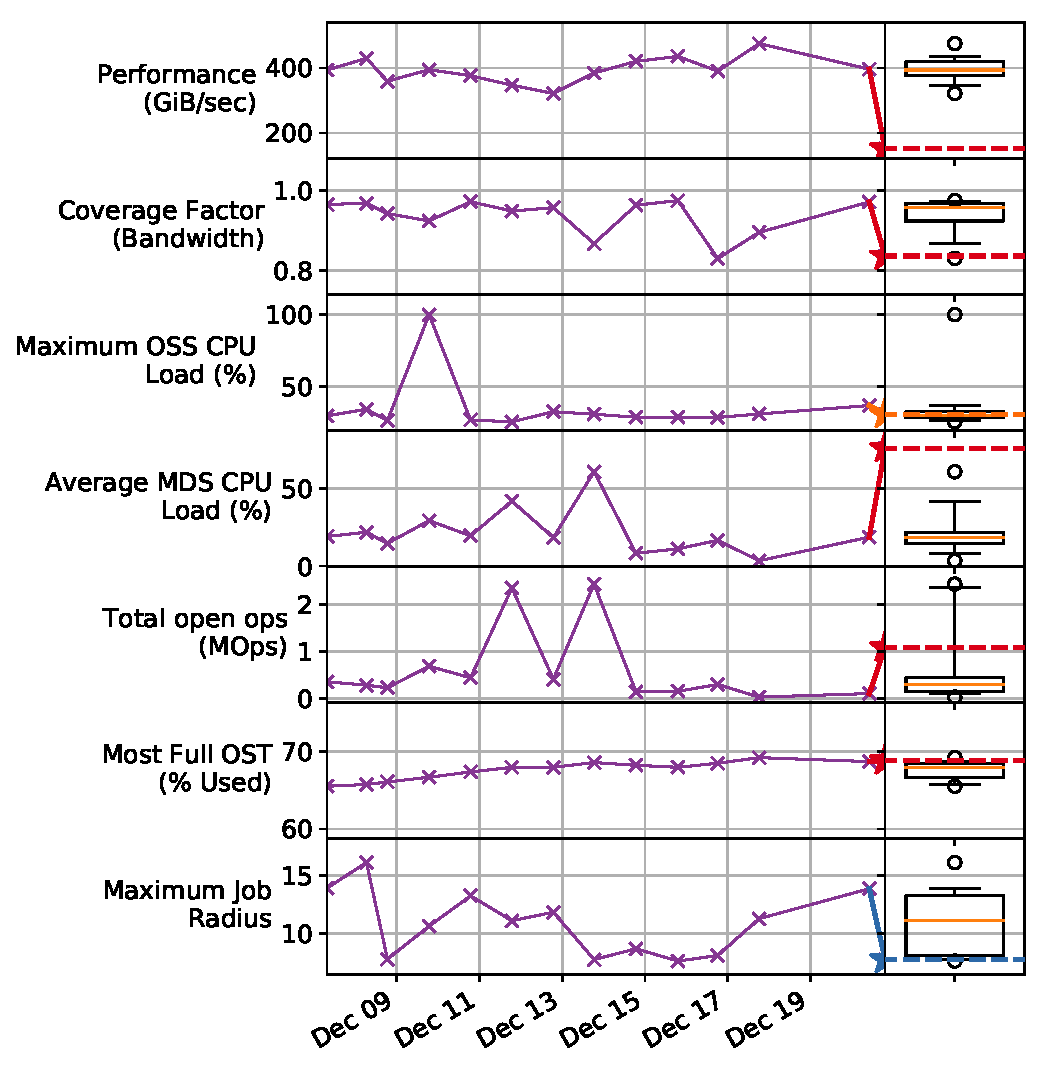
\includegraphics[width=1.0\columnwidth]{umami}
    \vspace{-.3in}
    \caption{UMAMI diagram of a simulated science campaign of HACC~\cite{Habib2012} simulations performed on NERSC's Cori system.  "Coverage Factor (Bandwidth)" is the fraction of global file system traffic originating from each HACC job, "Maximum Job Radius" represents the overall spread of each job's allocated nodes across the dragonfly network, and the remaining metrics represent server-side Lustre loads.}
    \label{fig:umami}
    \vspace{-.2in}
\end{figure}

pytokio also includes analyses to visualize systematic performance problems.  Figure \ref{fig:lustre-heatmap} shows the output of pytokio's OST load visualizer which revealed that poor stage-out performance from DataWarp to Lustre (which occurs outside the purview of user applications) resulted from poor Lustre striping.  By using pytokio's connector abstractions, both of these analyses were implemented in only several dozen lines of code.

\begin{figure}[t]
    \centering
    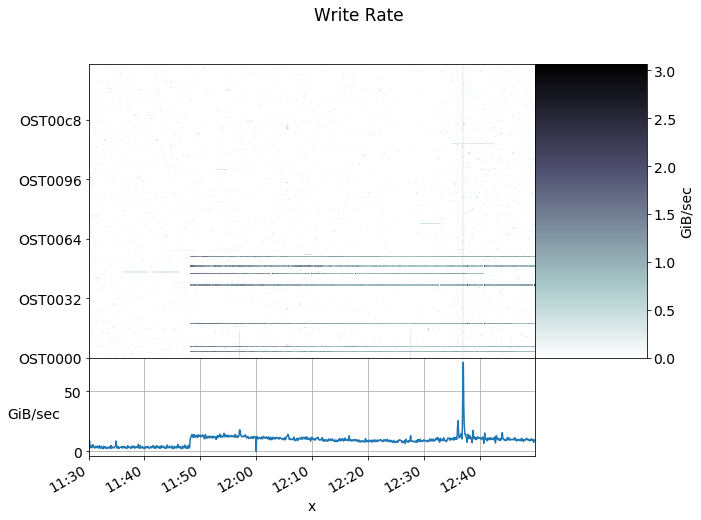
\includegraphics[width=1.0\columnwidth]{lustre-stageout-performance}
    \vspace{-.3in}
    \caption{Write rates of a stage-out operation from DataWarp to Lustre on Cori.  Each horizontal line represents a single OST performing intense I/O and whitespace is OST inactivity.  This visualization prompted the user to manually pre-stripe the DataWarp stage-out destination directory to ensure that the performance of all OSTs was available for subsequent stage-outs.}
    \label{fig:lustre-heatmap}
    \vspace{-.2in}
\end{figure}

To demonstrate the simplicity of deploying pytokio on different Cray systems, results from both NERSC's Cori and ALCF's Theta systems will also be presented.  Furthermore, because pytokio is BSD-licensed, new connectors to site-specific tools can be developed to suit the needs of different centers.  Full pytokio source code, ready-to-deploy packages, and broadly useful analysis applications will all be referenced.